\documentclass[10pt,brazil,english]{article}
\usepackage{amsfonts}
\usepackage{infocomp}
\usepackage{times}
\usepackage{amsmath}
\usepackage{amssymb}
\usepackage[T1]{fontenc}
\usepackage[english, portuguese]{babel}
\addto\captionsportuguese{
\renewcommand{\figurename}{Figura}
\renewcommand{\tablename}{Tabela}
\renewcommand{\refname}{REFER\^{E}NCIAS}
}
\usepackage[utf8]{inputenc}
\usepackage{multirow}
\usepackage{lscape}
\usepackage{rotating}
\usepackage{setspace} % espacamento entre linhas
\usepackage[table,xcdraw]{xcolor}
\usepackage{scalefnt}
\usepackage{graphicx}
\usepackage{hyperref}
\usepackage{subfigure}
\usepackage{enumerate}
\usepackage{caption}
\usepackage[sort,compress]{cite}
\usepackage[alf,abnt-repeated-author-omit=yes,abnt-etal-list=0]{abntex2cite}	% Citações padrão ABNT
%%%%%%%%%%%%%%%%%%%%%%%%%%%%%%%%%%%%%%%%%%%%%%%%%%%%%%%%%
\usepackage{fancyhdr}
\usepackage{mathtools}
\setcounter{page}{118}
\fancyhead{ }
\lhead{}
\chead{\footnotesize TÍTULO DO ARTIG}
\rhead{}
\cfoot{Conex. Ci. e Tecnol. Fortaleza/CE, v. xx, n. y, p. zzz - www, nov. 2016}
\rfoot{\thepage}%Direita do Rodapé
\renewcommand{\headrulewidth}{1pt}% Traço horizontal no cabeçalho

%%%%%%%%%%%%%%%%%%%%%%%%%%%%%%%%%%%%%%%%%%%%%%%%%%%%%%%%%

\usepackage{rangecite}

%\hyphenation{po-pu-la-ri-za-ção re-gis-tros do-mi-na-do-ra vio-la pe-ram-bu-lam dou-tri-na-ria-men-te co-nhe-ce-rem Ad-mis-tra-ção fa-bri-car so-cie-da-de in-fe-rio-res vee-men-te-men-te si-tua-ção pon-tuais}

\sloppy
\renewcommand{\captionfont}{\footnotesize}
\renewcommand{\captionlabelfont}{\footnotesize \bfseries}
\newtheorem{exemplo}{Exemplo}
\title{TÍTULO DO ARTIGO}

\address{
$^{1}$Instituição 1 (SIGLA1) \\
$^{2}$Instituição 2 (SIGLA2)\\
$^{3}$Instituição 3 (SIGLA3)\\ \\
\url{xxxx@yyy.br},~ \url{zzzz@rrr.com}, \\ ~ \url{tyuoo@uuu.br},~ \url{qqqq@ifxx.edu.br}\\ \\ DOI: 10.21439/conexoes.v10ix.999}

\author{Autor 1$^{1}$, Autor 2$^{1}$, \\ Autor 3$^{2}$$^{,}$$^{3}$, Autor 4$^{3}$ }

\selectlanguage{english}

\abstract{Neste caso deve ser seguida a mesma formatação utilizada na preparação do Resumo, obviamente com texto em língua inglesa, separadas pelo ponto, conforme exemplo abaixo.  }

\keywords{Learning. Digital Technologies. Mathematical Modeling. Optimization.}

\selectlanguage{brazil}

\resumo {Em termos da organização do trabalho, a primeira página do artigo deve conter: o título do artigo; o Resumo e o Abstract. Estes elementos pré-textuais não deverão ultrapassar a primeira página. O título do trabalho deverá ter, no máximo, três linhas. O resumo do artigo final deverá ter de 100 a 250 palavras com fonte (Times New Roman, tamanho 10, justificado). No resumo inicie introduzindo o trabalho e declare o objetivo. Indique se o trabalho trata de uma pesquisa (experimental, levantamento, estudo de caso, estudo de campo, pesquisa-ação) ou de uma compilação bibliográfica. Sintetize a metodologia utilizada. Finalize apresentando resultados e contribuições. Classifique o trabalho com no mínimo três e no máximo cinco palavras-chave separadas pelo ponto, conforme exemplo abaixo. Outras instruções para a preparação do artigo completo são apresentadas ao longo deste texto. }

\palchaves{Trabalho científico. Formatação. Resumo. Artigo completo. Submissão.}


%\receivedate{July 19th, 2011}
%\acceptdate{September 1st, 2011}

\begin{document}
\pagestyle{fancy} % CABECALHOO

\maketitle
\newpage


\section{\uppercase{Instruções gerais para preparação do manuscrito do trabalho}}

A partir da segunda página sugere-se estruturar o texto nas seguintes sessões, respeitada a natureza da área de conhecimento:

\begin{itemize}
\item \textbf{Introdução} (incluindo os componentes de revisão da literatura);
\item	\textbf{Fundamentação} (quando necessária ao desenvolvimento do estudo proposto);
\item	\textbf{Metodologia} ou Materiais e Métodos (quando houver);
\item	\textbf{Resultados} e Discussão (quando houver);
\item	\textbf{Conclusões} ou Considerações Finais;
\item	\textbf{Referências Bibliográficas}
\item	Outros elementos pós-textuais como agradecimentos, apêndices e anexos são opcionais.

\end{itemize}

Nesta parte são apresentadas as principais diretrizes para a elaboração do artigo completo no que diz respeito à apresentação gráfica, à estrutura e ao procedimento para a submissão do artigo. Este documento já possui a formatação de estilos personalizados para a elaboração do texto. O autor pode, portanto, utilizar este arquivo como modelo para esta finalidade.

O artigo completo deve conter no mínimo 10 páginas e no máximo 15 páginas. Os arquivos para submissão deverão estar no formato Microsoft Word (doc; docx) ou OpenOffice.Tabelas e figuras devem ser apresentadas ao longo do corpo do texto, porém como forma de otimizar ao máximo o conteúdo de cada página, as mesmas podem estar deslocadas.

O texto deve ser configurado em folha do tamanho A4 (210x297mm), incluindo a numeração de página indicada. A margem esquerda e superior deverá possuir 3 cm, enquanto que as demais margens (inferior e direita) deverão possuir 2 cm. No caso de citações de mais de três linhas, deve-se observar também um recuo de 4 cm da margem esquerda. Procure utilizar toda a área disponível. Exceções podem ser admitidas, por exemplo, quando for necessário começar uma nova seção, título, subtítulo ou legenda, esses poderão ser alocados no início da página seguinte.

\subsection{Fontes e Formatação}

Os textos deverão ser escritos em fonte (\textbf{Times New Roman, tamanho 12, justificado}) à exceção das citações com mais de três linhas, notas de rodapé, paginação, legendas e fontes das ilustrações e das tabelas, que devem ser em tamanho 10 e uniforme. Os títulos das seções devem estar apresentados em negrito, todo em maiúsculo (Estilo Título 1). Subtítulos em negrito devem apresentar somente apenas as primeiras letras de cada palavra em maiúscula (Estilo Título 1.1). Texto normal, espaço simples, sem recuo na primeira linha.

\section{\uppercase {Teste de seção}}
\subsection{Teste de subseção}
\subsubsection{Teste de subsubseção}

Testando subsubseção

\section{\uppercase{Espaçamento e parágrafos}}

Empregar espaçamento \textbf{simples}. Antes de um título principal (item 1) ou de figuras deverá ser deixado espaço em branco equivalente a duas linhas. Antes de um título secundário (1.1 ou 1.1.1) deverá ser deixado espaço em branco equivalente a uma linha). Se forem adotados os estilos deste arquivo de instruções, esses espaçamentos todos já estão previstos. Na formatação dos parágrafos escolher a opção \textbf{parágrafo justificado}. Este formato já está definido no presente arquivo de instruções.

\section{\uppercase{Equações}}

Para equações serão adotadas as unidades do Sistema Internacional (SI). As equações deverão estar separadas por linha adicional antes e depois, ser centralizadas e numeradas sequencialmente,

\begin{equation}
E=m.c^{2}
\label{Eq1}
\end{equation}

Na Equação \ref{Eq1} é apresentada a famosa equação de equivalência entre massa e energia de Eistein.

\section{\uppercase{Figuras e tabelas}}

As figuras serão inseridas no interior do texto, preferencialmente em seguida aos parágrafos a que se referem. Uma menção às figuras no texto corrido é necessária para a orientação do leitor. As figuras devem conter todos os elementos de formatação e de conteúdo para que sejam interpretadas corretamente, sem necessidade de se recorrer ao texto corrido para uma busca de informações adicionais. É importante observar as margens e o número máximo de páginas. As figuras e tabelas deverão ser centralizadas e numeradas sequencialmente. O número das figuras (ver Figura \ref{Fig1}) e das tabelas (ver Tabela \ref{Tab1}), seguido do título, devem aparecer na parte superior das mesmas, centralizado e negrito (tamanho 12). Separar do texto as tabelas e figuras com \textbf{1 linha} antes e depois. Fonte e legenda em tabelas e figuras devem ser apresentadas logo abaixo das mesmas (tamanho 10).

Evite utilizar letras, legendas e símbolos de pequenas dimensões. Para não comprometer a leitura não \textbf{empregar letras menores que tamanho 10} ou linhas muito finas. Utilizar fotografias somente quando forem imprescindíveis para a compreensão do texto. Recomenda-se que gráficos, figuras, fotos e qualquer arquivo gráfico, estejam inseridos no texto em formato ``jpg'' ou ``png''.


\begin{figure}[!hbtp]
\begin{center}

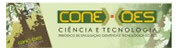
\includegraphics[scale=1]{figura.png}
\end{center}
\caption{Imagem da revista do IFCE. Fonte: (quando houver) inserir texto nesta posição.}
\label{Fig1}
\end{figure}


\begin{table}[!hbtp]
\centering
\caption{Estilos a serem utilizados.}
\label{Tab1}
\begin{tabular}{c|l|l|l|c}
\hline
\multirow{3}{*}{\textbf{Elemento}} & \multirow{3}{*}{\textbf{}} & \multicolumn{2}{l|}{\multirow{2}{*}{\textbf{}}} & \multirow{3}{*}{\textbf{Alinhamento}} \\
                                   &                            & \multicolumn{2}{l|}{}                           &                                       \\ \cline{3-4}
                                   &                            &                        &                        &                                       \\ \hline
Título do artigo                   &                            &                        &                        & Centralizado                          \\ \hline
Nome dos Autores                   &                            &                        &                        & Centralizado                          \\ \hline
Identificação dos autores          &                            &                        &                        & Centralizado                          \\ \hline
Título do resumo                   &                            &                        &                        & Esquerdo                              \\ \hline
Resumo                             &                            &                        &                        & Justificado                           \\ \hline
Palavras-chave                     &                            &                        &                        & Esquerdo                              \\ \hline
Título de Sessão                   &                            &                        &                        & Esquerdo                              \\ \hline
Título de subseção                 &                            &                        &                        & Esquerdo                              \\ \hline
Texto                              &                            &                        &                        & Justificado                           \\ \hline
Título de Figura e Tabela          &                            &                        &                        & Centralizado                          \\ \hline
Nota de rodapé                     &                            &                        &                        & Justificado                           \\ \hline
\end{tabular}

\end{table}



\section{\uppercase{Citações e referências}}

A qualidade técnico-científica do trabalho será um dos critérios de avaliação do artigo completo. Como já colocado anteriormente o autor deverá apresentar conceitos corretos, ter profundidade na abordagem teórica, rigor científico e fazer citação de referências fundamentais para o tema utilizando a NBR10520 da ASSOCIAÇÃO BRASILEIRA DE NORMAS TÉCNICAS. Evitar citações diretas. \textbf{As referências bibliográficas devem ser listadas em ordem alfabética.} Toda referência deve ser citada seguindo a NBR6023 da ASSOCIAÇÃO BRASILEIRA DE NORMAS TÉCNICAS. Sendo assim, apresentaremos a seguir alguns exemplos de utilização:

\begin{itemize}
\item \nocite{Brasil2002} - sem citação, só referência, usar \textit{nocite{}};
\item \cite{dana2010integral} - citação indireta;
\item \citeonline{dana2010integral} - citação direta.
\end{itemize}

\begin{itemize}
\item Artigo em jornal ou revista, paper \cite{dana2010integral};
\item Livro \cite{Lima2004};
\item Lei ou decreto: \cite{BrasilEAD2005};
\item Link de internet \cite{Reis2012};
\item Capítulo de livro \cite{Medeiros2005};
\item Tese \cite{Tome2011} e dissertação \cite{Hsia2006};
\item Artigo em anais de evento \cite{Gonzalez2005};
\end{itemize}

\subsection{Citação direta com recuo}

Um exemplo \citeonline{santos2011} é apresentado:

\begin{quote} \footnotesize
``Acreditamos que o revigoramento da qualidade da educação está intimamente associado aos processos de ensino e aprendizagem. Nesta direção, focamos a realidade vivenciada em sala de aula, no tocante ao estabelecimento de articulações entre teoria e prática, repensando-se os caminhos da prática pedagógica e o desenvolvimento cooperativo do processo de aprendizagem significativa e de construção de novos conhecimentos'' \cite[p. 254]{santos2011}.
\end{quote}




\bibliography{Referencias}

%\anex
%\begin{anexosenv}
%\onecolumn
% ---



\end{document} 